\documentclass[a4paper]{article}
\usepackage[fontsize=13pt]{scrextend}
\usepackage[margin=1in]{geometry}
\usepackage[T1]{fontenc}
\usepackage[utf8]{inputenc}
\usepackage{lmodern}
\usepackage{setspace}
\usepackage{hyperref}
\usepackage{algorithm}
\usepackage{algpseudocode}
\usepackage{amsmath}
\usepackage{booktabs}
\usepackage{amssymb}
\usepackage{tikz}
\usepackage{float}

\usetikzlibrary{positioning, arrows.meta}
\setstretch{1.2}

\title{Methodology}
\author{}
\date{}

\begin{document}
\maketitle

This chapter defines the experimental methodology for evaluating schema injection and evidence-condition effects on RealHiTBench. It presents the ablation design and condition definitions, the table information-extraction pipeline, the two-stage evaluation protocol, and the validity analysis.

\section{Research Design}

This chapter presents the experimental methodology of the thesis
and is organized around two main contributions. The first is a
benchmark audit and dataset-finalization procedure that produces a
cleaned RealHiTBench subset through three-reviewer verification,
agreement analysis, and majority-vote resolution. The second is a
table processing and schema-injection pipeline that transforms raw
hierarchical HTML tables into explicit structural evidence for LLM
prompting. Building on these two components, the chapter then
defines the ablation conditions, evaluation protocol, and validity
boundaries used throughout the study.

\subsection{Research Questions}

\textbf{RQ1:} Does hierarchical schema injection improve LLM answer accuracy on RealHiTBench relative to a raw-HTML baseline when all other inference settings are held constant?

\textbf{RQ2:} Within schema-injected settings, does adding an explicit evidence-oriented reasoning scaffold further improve LLM answer accuracy relative to schema injection alone?

\section{Benchmark Audit and Dataset Finalization}

Reliable ablation results require reliable reference answers. In hierarchical table QA this requirement is non-trivial: deriving the correct answer often demands navigating multi-level headers, resolving merged-cell scope, and performing arithmetic over cells that are only identifiable through structural inference. Annotation errors in the gold standard---whether incorrect computations, misidentified header regions, or references to the wrong table---propagate directly into false negatives under exact match and can reverse the sign of a condition contrast. Before any comparative run was executed, the study therefore conducted a systematic audit of the RealHiTBench gold answers to separate genuine model errors from benchmark noise.

An initial pilot batch of the first $100$ question--table pairs under a single condition confirmed two concerns. First, a subset of gold answers were inconsistent with the values derivable from the linked table, suggesting annotation noise in the original reference set. Second, normalized exact match penalized formatting differences, unit variations, and numerically equivalent representations that a human reader would accept as correct. Because both concerns affected the reliability of condition-level comparisons, the study expanded the audit to cover the full candidate set of $771$ items before locking the evaluation protocol.

\subsection{Annotation Protocol and Label Space}

Three independent reviewers each received a spreadsheet containing the question text, the linked table source, and the original benchmark gold answer (the ``Processed Answer''). For each item, the reviewer located the corresponding table, independently derived an answer from the table evidence, and recorded one of three categorical responses. Formally, let the label space be $L = \{\textsc{Agree}, \textsc{Correct}, \textsc{Invalid}\}$, where each reviewer $j \in \{1, 2, 3\}$ assigns a label $l_{i,j} \in L$ for question $i$:

\begin{enumerate}
    \item \textbf{\textsc{Agree}:} The original gold answer is correct. Coded as \texttt{Match} or \texttt{X} in the annotation spreadsheet; both tags were treated as equivalent for coding purposes.
    \item \textbf{\textsc{Correct}:} The original gold answer is incorrect, but the question is answerable. The reviewer supplies the corrected answer as a free-text string.
    \item \textbf{\textsc{Invalid}:} The question is unanswerable from the provided table. Coded as \texttt{NO INFO} or \texttt{wrong table}, indicating missing data or a broken table link.
\end{enumerate}

All reviewer responses were finalized independently before any cross-consultation or exposure to other reviewers' labels.

\subsection{Inter-Rater Agreement}

Inter-rater reliability was measured using Fleiss' $\kappa$ over the three-category label space ($k = 3$) across all $N = 771$ items with $n = 3$ raters per item. Observed pairwise agreement was $\bar{P} = 0.852$ and chance-expected agreement was $\bar{P}_e = 0.711$, yielding

\[
\kappa = \frac{\bar{P} - \bar{P}_e}{1 - \bar{P}_e} = \frac{0.852 - 0.711}{1 - 0.711} = 0.49
\]

\noindent which corresponds to \emph{moderate} agreement on the Landis and Koch scale. The category-level marginals were $p_{\textsc{Agree}} = 0.831$, $p_{\textsc{Correct}} = 0.145$, and $p_{\textsc{Invalid}} = 0.025$, indicating that the large majority of gold answers were endorsed by all three reviewers, and that disagreement was concentrated in the correction and invalidation categories.

A $\kappa$ of $0.49$ is consistent with the inherent difficulty of hierarchical table annotation: many RealHiTBench questions require multi-step arithmetic over cells identified through nested header paths, and reviewers can legitimately reach different numerical results depending on which cells they include within a merged-header scope. The moderate agreement thus reflects genuine task ambiguity rather than rater carelessness, and motivates the strict consensus requirement imposed by the voting protocol described below.

\subsection{Majority Voting and Exclusion Protocol}

The finalized gold answer for each item was determined by strict majority voting. For question $i$, define the multiset of reviewer labels as $V_i = \{l_{i,1},\; l_{i,2},\; l_{i,3}\}$. Resolution proceeds as follows:

\begin{enumerate}
    \item \textbf{Majority consensus ($\ge 2$ identical labels):} If any label $v$ satisfies $\mathrm{count}(v, V_i) \ge 2$, that label determines the outcome. If the majority is \textsc{Agree}, the original gold answer is retained. If the majority is \textsc{Correct} and the two (or three) correcting reviewers supply the same replacement string, that string becomes the locked gold answer. If the majority is \textsc{Invalid}, the item is excluded as unanswerable.
    \item \textbf{Majority correction with divergent values:} If two or more reviewers label the item \textsc{Correct} but supply numerically distinct replacement strings, no single answer commands consensus. These items are excluded.
    \item \textbf{Complete three-way disagreement ($|V_i| = 3$ distinct labels):} Items on which all three reviewers produce mutually distinct responses---e.g., one agreement, one correction, and one invalidation---are excluded as irreducibly ambiguous.
\end{enumerate}

\subsection{Audit Outcome}

Of the $771$ items audited, $663$ received majority \textsc{Agree} (original gold answer retained), $63$ received majority \textsc{Correct} with a single converged replacement answer, and $46$ were excluded from the evaluation subset. The exclusions decompose as follows: $27$ items had majority \textsc{Correct} but with divergent corrected values across reviewers, $14$ were majority \textsc{Invalid} (unanswerable due to missing data or broken table links), $4$ exhibited complete three-way disagreement, and $1$ was excluded on manual inspection. The resulting cleaned subset comprises $N = 726$ question--table pairs, each backed by a consensus-endorsed reference answer traceable to the table evidence.

The cleaned RealHiTBench subset constitutes a secondary contribution of this thesis: a verified, majority-voted gold-standard benchmark for hierarchical table QA that future work can reuse without re-auditing. Both the cleaned reference file and the per-item reviewer annotations are released alongside this thesis.

The audit also directly motivated the two-stage evaluation design adopted throughout the study. The observation that exact match penalized semantically correct but surface-mismatched answers led to the decision to retain normalized exact match as a deterministic first-stage diagnostic while escalating all exact-match failures to evidence-based LLM adjudication (Section~\ref{sec:evaluation}). Following the conclusion of the audit, both the cleaned benchmark subset and the scoring procedure were locked and applied uniformly across all reported condition runs.

\section{Table Processing Pipeline}

Hierarchical Table Question Answering poses a particular challenge for LLMs because correct answering depends not only on reading cell values, but also on inferring the correct navigational path through the table structure. In hierarchical tables, relevant information is often distributed across multi-level row and column headers, merged cells, and indentation-based groupings. To answer a question correctly, the model must first identify which structural route connects the question to the relevant cell or set of cells, and only then retrieve or compute the answer. When this structure is left implicit in raw HTML, the model must reconstruct it from visual layout cues alone, which is error-prone in nested or irregular tables.

The table processing pipeline is designed to reduce this burden by converting raw hierarchical tables into prompt-ready evidence that makes structural organization explicit before inference. Rather than requiring the model to infer header scope and row grouping implicitly, the pipeline extracts serialized column and row root-to-leaf paths together with canonicalized table content. These structural cues act as prior navigational information: they expose how local labels are situated within the full hierarchy and help the model align the question with the correct region of the table. In this way, the pipeline supports more reliable table navigation and reduces errors caused by ambiguity or visually encoded structure.

\subsection{Stage Overview}

The pipeline operates in four stages:
\begin{figure}[H] % Use figure* if you need it to span two columns in an ACL format
\centering
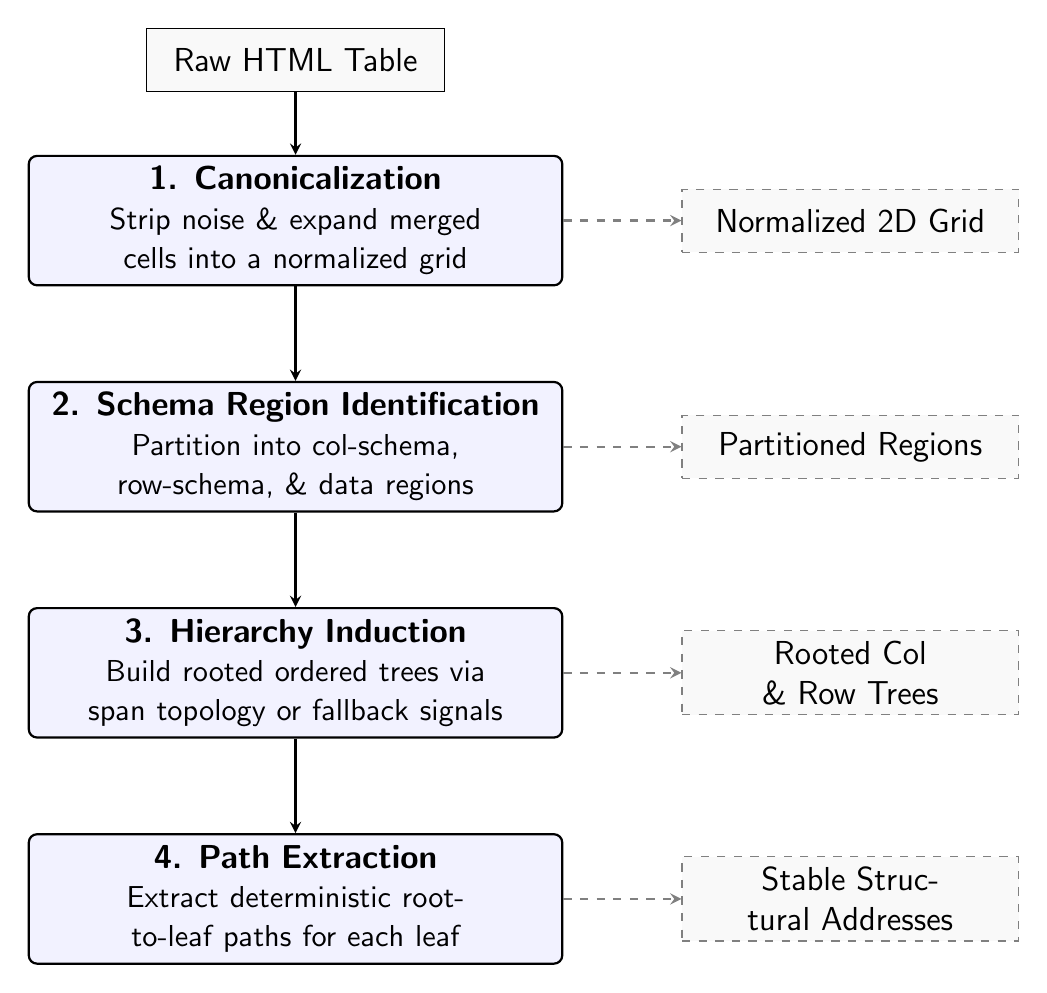
\begin{tikzpicture}[
    node distance=1.2cm and 1.5cm,
    font=\sffamily\small,
    % Define styles for consistent blocks
    process/.style={rectangle, draw=black, thick, fill=blue!5, text width=6.5cm, align=center, minimum height=1.4cm, rounded corners=3pt},
    artifact/.style={rectangle, draw=gray, dashed, fill=gray!5, text width=4cm, align=center, minimum height=0.8cm},
    arrow/.style={->, thick, >=stealth}
]

% --- Nodes ---

% Input
\node[artifact, text width=3.5cm, draw=black, solid] (input) {Raw HTML Table};

% Step 1
\node[process, below=0.8cm of input] (p1) {\textbf{1. Canonicalization} \\ \footnotesize Strip noise \& expand merged cells into a normalized grid};
\node[artifact, right=of p1] (a1) {Normalized 2D Grid};

% Step 2
\node[process, below=of p1] (p2) {\textbf{2. Schema Region Identification} \\ \footnotesize Partition into col-schema, row-schema, \& data regions};
\node[artifact, right=of p2] (a2) {Partitioned Regions};

% Step 3
\node[process, below=of p2] (p3) {\textbf{3. Hierarchy Induction} \\ \footnotesize Build rooted ordered trees via span topology or fallback signals};
\node[artifact, right=of p3] (a3) {Rooted Col \& Row Trees};

% Step 4
\node[process, below=of p3] (p4) {\textbf{4. Path Extraction} \\ \footnotesize Extract deterministic root-to-leaf paths for each leaf};
\node[artifact, right=of p4] (a4) {Stable Structural Addresses};


% --- Routing Arrows ---

% Main flow
\draw[arrow] (input) -- (p1);
\draw[arrow] (p1) -- (p2);
\draw[arrow] (p2) -- (p3);
\draw[arrow] (p3) -- (p4);

% Data artifacts flow
\draw[->, thick, dashed, draw=gray, >=stealth] (p1) -- (a1);
\draw[->, thick, dashed, draw=gray, >=stealth] (p2) -- (a2);
\draw[->, thick, dashed, draw=gray, >=stealth] (p3) -- (a3);
\draw[->, thick, dashed, draw=gray, >=stealth] (p4) -- (a4);

\end{tikzpicture}
\caption{The four-stage table processing pipeline. Raw HTML layout is deterministically transformed into explicit structural addresses before LLM reasoning.}
\label{fig:pipeline_overview}
\end{figure}


\subsection{Implementation Details}

\textit{Canonicalization.} Non-semantic HTML artifacts—such as style tags, decorative wrappers, empty spacer cells, and footnote markers—are stripped to maximize token efficiency within the LLM context window while preserving deterministic reading order. Furthermore, because RealHiTBench frequently encodes hierarchical relations through visual cell-merging (\texttt{colspan} and \texttt{rowspan}) rather than explicit semantic markup, these spans must be explicitly resolved. Each merged-cell value is broadcast across all covered positions, transforming the irregular HTML table into the strict, normalized two-dimensional grid required for downstream schema extraction.

\textit{Schema region identification.} The normalized grid is partitioned into a column-schema region, a row-schema region, and a data region. The column-schema region is identified as the topmost contiguous band of rows in which at least one of the following header criteria is satisfied: all cells are encapsulated by \texttt{<th>} tags, any cell utilizes \texttt{rowspan} or \texttt{colspan} attributes, or at most one-third of the non-empty cells evaluate as numeric. The row-schema region is similarly identified as the leftmost contiguous band of columns where at most one-third of non-empty cells evaluate as numeric, computed after the column-schema rows have been excluded. Data cells---defined as numeric, monetary, or short alphanumeric values expected to vary across rows---are isolated from both schema regions. This explicit partitioning prevents the model from prematurely ingesting values before it has acquired sufficient structural context.

\textit{Hierarchy induction.} We construct hierarchical trees for both columns and rows. Because RealHiTBench tables vary heavily in how they format headers, the pipeline prioritizes explicit HTML tags and falls back to visual layout cues when tags are absent.

\textbf{Column hierarchy:} If the parsed HTML contains explicit \texttt{colspan} attributes, parent--child relationships are derived directly from these boundaries: a cell spanning columns $[l, r]$ in row $i$ becomes the parent of the cells in row $i{+}1$ that fall within that same $[l, r]$ range. If span attributes are missing, the pipeline defaults to reading the header labels top-to-bottom to extract each column's path.

\textbf{Row hierarchy:} If the row-schema region spans multiple columns, the hierarchy is extracted by reading left-to-right. If the region is only a single column wide, the pipeline infers depth from text indentation by counting leading space characters (after normalizing HTML non-breaking spaces). These space counts are sorted and mapped to discrete depth levels $\{0, 1, \ldots, d\}$. If no indentation is present, all rows are treated as a flat list at depth 0.

\subsection{Transformation Trace}

The pipeline executes in the following fixed order so that each intermediate output is inspectable:
\begin{enumerate}
\item Read the linked raw HTML table and retain table-relevant context.
\item Remove non-semantic markup while preserving cell text and reading order.
\item Resolve row-span and column-span relations into a normalized grid.
\item Partition the grid into column-schema, row-schema, and data regions.
\item Build column and row hierarchy trees from the schema regions.
\item Extract and normalize root-to-leaf paths for both hierarchies.
\item Serialize structural evidence and pair it with cleaned table content according to the target condition (\(C1\), \(C2\), or \(C3\)).
\end{enumerate}

Tables that fail width, leaf-count, or path-uniqueness consistency checks are flagged for manual audit before inference. Flagged items are inspected, and the audit outcome is recorded: repaired items re-enter the pipeline, excluded items are counted and reported, and if no items were excluded, that fact is stated explicitly in the results.

Example serialized schema: \texttt{Column paths: [Age > Male, Age > Female]; Row paths: [Region > Urban, Region > Rural]}.

\subsection{Condition-Specific Prompt Exposure}

The extracted structural representation is identical across all executed conditions; only its exposure within the prompt varies. In \(C1\), the model receives cleaned table HTML and the question only. In \(C2\), the model additionally receives the extracted column and row paths. In \(C3\), the same structural evidence is provided together with an explicit evidence-oriented reasoning scaffold. Accordingly, \(C1\) versus \(C2\) isolates the effect of schema exposure, while \(C2\) versus \(C3\) isolates the incremental effect of the reasoning scaffold once schema is already available.

\section{Ablation Conditions}

The ablation isolates which component of the proposed method drives 
any observed performance change. The design is cumulative: each 
successive condition adds one structural or reasoning component while 
holding all other inference settings constant. Conditions are labeled 
C1, C2, and C3; the gaps in numbering reflect intermediate pilot 
variants explored during development that were not carried forward 
into the final design.

\subsection{Condition Definitions}

Canonicalization --- noise stripping and merged-cell resolution --- 
is applied as a shared preprocessing step uniformly across all 
executed conditions. Its contribution is not separately estimated; 
the ablation isolates the effect of schema injection and reasoning 
scaffolding given a preprocessed representation. A raw-HTML 
diagnostic (Section~\ref{sec:rawhtml}) is reported separately as a 
sanity check confirming that preprocessing provides a non-trivial 
baseline improvement.

\begin{enumerate}
    \item \textbf{C0:} Benchmark-anchor baseline reported by 
    RealHiTBench; not executed in the present study and included 
    only as an external reference point for absolute score 
    comparability with the published leaderboard.

    \item \textbf{C1:} Preprocessing-matched baseline. The model 
    receives cleaned table HTML and the question, with no schema 
    injection or reasoning scaffold. Canonicalization is already 
    applied at this stage; C1 therefore serves as a 
    preprocessing-matched rather than raw-HTML baseline.

    \item \textbf{C2:} Schema-injection condition. The model receives 
    cleaned table HTML together with extracted column and row 
    hierarchy paths, but follows no enforced reasoning pipeline.

    \item \textbf{C3:} Full-method condition. The model receives 
    cleaned table HTML, extracted hierarchical schema, and an 
    explicit evidence-driven reasoning scaffold requiring schema 
    orientation, value extraction, computation, and validation 
    before stating the final answer.
\end{enumerate}

The ablation factor is therefore a controlled manipulation of 
structural evidence and reasoning-scaffold constraints at inference 
time, not merely prompt wording. \(C1\) versus \(C2\) estimates the 
effect of schema injection given preprocessing (RQ1), while \(C2\) 
versus \(C3\) estimates the incremental effect of adding an explicit 
reasoning scaffold when schema is already available (RQ2). The 
present design does not estimate the effect of reasoning scaffolding 
in the absence of schema injection.

\subsection{External Comparison: TreeThinker}

Beyond the internal ablation, the full method (C3) is additionally 
evaluated against TreeThinker~\cite{wu2025realhitbench}, the 
pipeline proposed by the RealHiTBench benchmark authors and 
therefore the most relevant prior baseline on this benchmark. 
TreeThinker organizes hierarchical headers into a tree structure 
via a multi-turn React-style prompting loop (Thought, Action, 
Result), requiring multiple sequential inference passes per 
question. The present method differs in that schema extraction is 
deterministic and single-pass rather than model-driven and 
multi-turn.

For the TreeThinker comparison to be methodologically controlled, 
TreeThinker was re-executed on the same audited subset under 
identical conditions: the same base model, the same normalized 
exact-match scoring procedure, and the same two-stage evaluation 
protocol as the internal ablation conditions. This pairing makes 
the C3 versus TreeThinker contrast directly comparable to the 
internal ablation contrasts, and McNemar's exact test is applied 
to assess statistical significance, consistent with the analysis 
plan for RQ1 and RQ2.

\subsection{Condition Contrast Matrix}

To make condition differences auditable, 
Table~\ref{tab:condition-contrast} states exactly which components 
change across conditions. TreeThinker is included as an external 
row for completeness.

\begin{table}[h]
\centering
\caption{Condition-wise component differences. TreeThinker is an 
external comparison and is not part of the internal ablation.}
\label{tab:condition-contrast}
\begin{tabular}{lcccc}
\toprule
\textbf{Condition} & \textbf{Cleaned HTML} & \textbf{Injected Schema} 
    & \textbf{Reasoning Scaffold} & \textbf{Type} \\
\midrule
C0                 & \multicolumn{3}{c}{benchmark-defined} 
    & external ref. \\
C1                 & $\checkmark$ & --           & -- 
    & internal \\
C2                 & $\checkmark$ & $\checkmark$ & -- 
    & internal \\
C3                 & $\checkmark$ & $\checkmark$ & $\checkmark$ 
    & internal \\
TreeThinker        & $\checkmark$ & $\checkmark$ & multi-turn loop 
    & external \\
\bottomrule
\end{tabular}
\end{table}

\subsection{Prompt Exposure Per Condition}

The structural representation produced by the pipeline is identical 
across all executed conditions; only its exposure within the prompt 
varies. In \(C1\), the model receives cleaned table HTML and the 
question only. In \(C2\), the model additionally receives the 
extracted column and row hierarchy paths. In \(C3\), the same 
structural evidence is provided together with an explicit 
evidence-oriented reasoning scaffold. Accordingly, \(C1\) versus 
\(C2\) isolates the effect of schema exposure, while \(C2\) versus 
\(C3\) isolates the incremental effect of the reasoning scaffold 
once schema is already available.

\subsection{Execution Protocol}

Each experiment run is executed under one fixed condition, and 
every question in the audited subset is evaluated under that same 
condition. The same question set is reused across all runs --- 
including the TreeThinker re-execution --- so that all pairwise 
comparisons reflect only method differences, not dataset 
composition. Fixed-condition execution is preferred over 
per-question routing because routing would introduce assignment 
policy as a second intervention, confounding the isolation target 
of RQ1.

\section{Evaluation Protocol}
\label{sec:evaluation}

This section defines the two-stage evaluation protocol used to score model outputs across all executed conditions: normalized exact match as a deterministic first-pass diagnostic, followed by three-judge LLM adjudication for all items that fail exact match. This design was finalized after the audit observation that identified limitations in both the original gold answers and in purely lexical scoring. The subsections below present the benchmark audit, the exact-match scoring rules, the judge adjudication procedure, the formal definition of corrected accuracy, and the statistical analysis plan.

\subsection{Exact Match Scoring}

The study adopts the same answer normalization procedure used by the RealHiTBench benchmark to ensure comparability with reported benchmark scores. Normalized exact match applies the following deterministic transformations to both prediction and reference: trimming leading and trailing whitespace, removing outer quotation marks, stripping a trailing sentence period, removing currency symbols (\texttt{\$}), percentage markers (\texttt{\%}), and thousands separators (\texttt{,}), removing English articles (\textit{a}, \textit{an}, \textit{the}), replacing all remaining non-alphanumeric non-whitespace characters with a space, lowercasing, collapsing repeated whitespace, and canonicalizing numerically equivalent whole-number forms such as \texttt{7.0} $\to$ \texttt{7}. This normalization is deliberately inclusive: because all items that fail exact match are escalated to evidence-based LLM adjudication in the second stage, the first stage is designed to maximize recall of surface-form equivalences rather than to preserve fine-grained semantic distinctions. No semantic paraphrase normalization is applied at this stage.

\subsection{LLM Judge Adjudication}

All items with \(EM = 0\) are routed to the judge pipeline with no additional filtering threshold. Each judge receives the question, the gold answer, the model answer, and the condition-invariant cleaned table HTML (i.e., the \(C1\)-style representation---cleaned HTML without injected schema), together with a fixed judge prompt. Crucially, all conditions share the same judge context: the judge always sees the cleaned HTML rather than the condition-specific prompt representation. This design ensures that judge evidence does not vary across conditions and therefore cannot introduce a condition-dependent confound into adjudication.

The judge panel consists of three models---Claude Sonnet 4.6, GPT 5.4 Thinking, and Grok Expert---accessed through their respective web chat interfaces (claude.ai, chatgpt.com, and grok.x.ai). For each batch, the fixed judge prompt and the batch CSV were pasted into a new conversation; the model returned the same CSV with the \texttt{judgement} column filled. Because judging was conducted through chat interfaces rather than versioned API endpoints, the exact model checkpoint active at the time of each session is not recorded. Three judges are used because this is the minimum panel size that makes both Fleiss' Kappa and non-trivial majority voting well-defined while reducing dependence on any single model. Each judge returns one label from \{CORRECT, INCORRECT, UNCERTAIN\}. \texttt{UNCERTAIN} is treated as abstention.

Final adjudication follows majority vote over binary correctness labels: an item is marked \texttt{CORRECT} if at least two judges return \texttt{CORRECT}, and \texttt{INCORRECT} if at least two return \texttt{INCORRECT}. All remaining cases are marked \texttt{HUMAN\_REVIEW} and reported separately. Unless otherwise stated, unresolved cases are treated as non-correct outcomes in corrected-accuracy reporting. In the degenerate case where all three judges return \texttt{UNCERTAIN}, the item is marked \texttt{HUMAN\_REVIEW} and counted as incorrect in corrected-accuracy reporting; this is the most conservative possible outcome under the majority-vote rule.

Inter-rater reliability is assessed with Fleiss' Kappa over the three-judge label set, which is appropriate because agreement must be measured across more than two raters at the categorical-label level.

\subsection{Corrected Accuracy}

The primary outcome metric, corrected accuracy, combines exact match and judge adjudication into a single per-condition score. Let $Q$ be the set of $N$ questions evaluated under condition $s$. For each question $q_i$, define the corrected correctness indicator:
\[
\tilde{y}_i =
\begin{cases}
1 & \text{if } \mathrm{EM}(q_i) = 1, \\
1 & \text{if } \mathrm{EM}(q_i) = 0 \text{ and majority-vote label} = \texttt{CORRECT}, \\
0 & \text{otherwise (including } \texttt{HUMAN\_REVIEW}\text{).}
\end{cases}
\]
Corrected accuracy for condition $s$ is then:
\[
\mathrm{CA}(s) = \frac{1}{N} \sum_{i=1}^{N} \tilde{y}_i.
\]
This formulation ensures that EM-correct items are never sent to judges, that the judge stage only resolves the EM-failed subset, and that unresolved cases are treated conservatively as incorrect.

All answering runs use the provider API's default decoding temperature, held constant across all three executed conditions, and rely on provider defaults for all other decoding parameters (\texttt{top\_p}, \texttt{presence\_penalty}, \texttt{frequency\_penalty} are not overridden; \texttt{max\_tokens} is set to 32{,}000 to accommodate verbose chain-of-thought responses from \(C3\)). Holding temperature constant across conditions ensures that observed performance differences reflect evidence-condition effects rather than sampling variance. For non-exact-match cases, residual output variability is further mitigated by three-judge majority voting.

\subsection{Reproducibility Controls}

The evaluated conditions use fixed, version-controlled prompt templates with consistent section ordering across runs. The RealHiTBench question source is the audited subset file \texttt{tests/questions\_clean\_audit copy.jsonl}, reused across all conditions to preserve pairwise comparability. The exact answering templates for \(C1\), \(C2\), and \(C3\), together with the fixed judge prompt, are reproduced in Appendix~A for auditability. Because each scoring step is rule-based and condition-invariant, an independent evaluator can reproduce the scoring logic and executed protocol, given the released templates and scripts.

\subsection{Statistical Analysis Plan}

Because the same question set is evaluated under each condition, all comparisons are paired at the item level. The primary contrasts are \(C1\) versus \(C2\) (RQ1) and \(C2\) versus \(C3\) (RQ2). Statistical significance is assessed using McNemar's exact test (binomial) on paired correctness outcomes, and effect size is reported as the raw accuracy difference between conditions. Subtype-level analyses are treated as exploratory because several subtype sample sizes are limited.

Comparative claims are constrained to the executed conditions. \(C0\) is reported descriptively as a benchmark anchor; no inferential statistics are computed between \(C0\) and the executed conditions. Agreement statistics are computed on the same judge labels used for adjudication, so reliability reporting matches the actual decision mechanism.

\section{Validity and Limitations}
\label{sec:validity}
% ---------------------------------------------------------------

\textit{Schema extraction sensitivity.} The pipeline is 
deterministic but sensitive to irregular table layouts; tables 
failing structural consistency checks are flagged, inspected, 
and either repaired or excluded before inference, with outcomes 
reported in Chapter~5.

\textit{Preprocessing scope.} The ablation isolates schema 
injection and reasoning scaffolding given a preprocessed 
representation; the independent contribution of canonicalization 
is not estimated and remains a direction for future work.

\textit{LLM-as-judge uncertainty.} Judge labels are 
model-mediated rather than human-verified. Three-model 
independent judging with majority aggregation and Fleiss' Kappa 
reporting mitigates but does not eliminate this risk.

\textit{Judge version pinning.} Judges were accessed via web 
chat interfaces; exact model checkpoints at the time of each 
session are not recorded, limiting strict reproducibility of the 
adjudication stage.

\textit{Single-benchmark domain.} All conditions are evaluated 
on one dataset. Relative condition effects are valid within 
RealHiTBench but do not generalize to other benchmarks without 
replication.

\textit{Subtype underpowering.} Some reasoning subtype sample 
sizes are small; subtype-level results are reported as 
exploratory, not confirmatory.

The valid claim scope of this thesis is condition-wise 
comparative performance on the audited RealHiTBench subset under 
the stated protocol. Results are reported in Chapter~5.

\subsection{Claim Boundary}

The valid claim scope of this thesis is limited to condition-wise comparative performance on the evaluated RealHiTBench subset under the stated scoring and adjudication protocol. Conclusions are interpreted as within-benchmark evidence for schema injection and reasoning-scaffold effects, not as dataset-independent or model-independent guarantees.

The results of applying this methodology across \(C1\), \(C2\), and \(C3\), with \(C0\) as a benchmark anchor, are reported in Chapter~5.

\end{document}







